\section{Machine Learning}\label{ml}
\subsection{Sighting Number Regression}
In order to predict how many sightings may occur in the future, we try to find the relations between the number of sightings and other macro factors, such as area, year and population data. Figure \ref{year} shows detailed distribution of numbers of sightings from 1986 to 2016, while figure \ref{regression} shows how the number of sightings and $ln(population)$ varies relatively. It is clear that the overall number of sightings has been increasing during the last 60 years, although slightly decreased recently. However, we find there is little correlation between states' area and the numbers of their sighting reports after analyzing them thoroughly.
\begin{figure}[H]
    \centering
    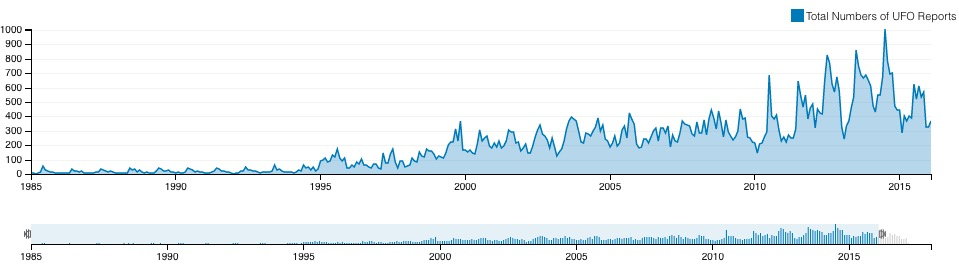
\includegraphics[width=17cm]{figure/year.jpg}
    \caption{sighting number}
    \label{year}
\end{figure}

\begin{figure}[H]
    \centering
    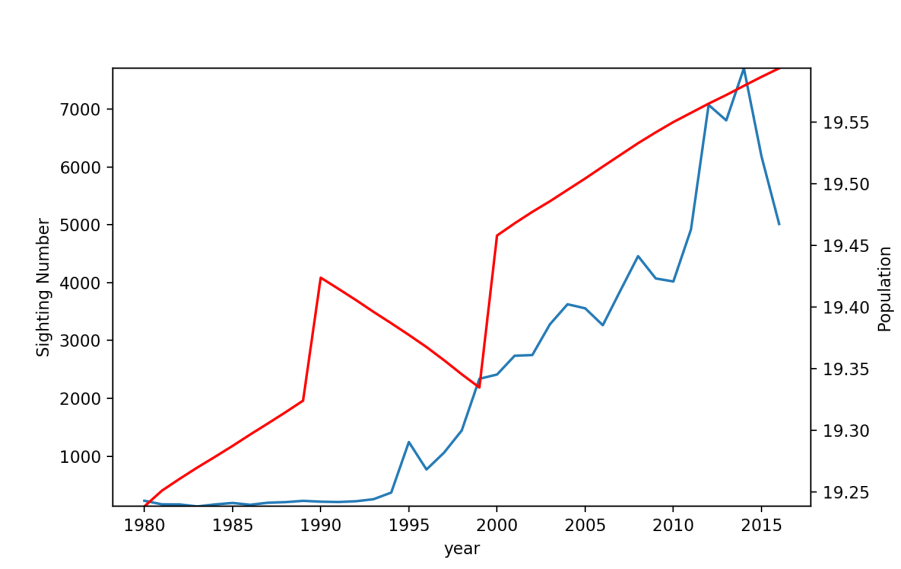
\includegraphics[width=10cm]{figure/regression.png}
    \caption{population and sighting number}
    \label{regression}
\end{figure}

We use four degree polynomial regression to fit year, total population of U.S. and total number of sightings. Generally, the result is perfect as our regression score is 0.96 out of 1. Given that the population of U.S. is 326474013 this year, we predict that there will be about 5589 UFO sightings across U.S. in 2017.

\subsection{Fake Detection}

We have encountered two main problems when working on fake detection. First, for each observation, there are two types of features --- text and numeric features, which is difficult to analyze at the same time or within the same classifier. Second, as described in section \ref{data}, each report is labeled by NUFORC's comment. However, since only a small proportion (about 5000) are labeled as fake, our data is extremely imbalanced.

To tackle the first problem, we use different classifiers for different features, and then combine all results together. After testing, we choose Decision Tree and SVM with RBF kernel to train numeric features, while using Logistic Regression and Decision Tree to train summary features. Other features, such as weather condition and shape of UFO, are quantified to numbers in order to train classifiers. For summary data, we use Porter Stemming algorithm to reduce data dimension, and then vectorize all words.

To solve the second problem, we design experiments to find out the best class weight for different classifiers. Changing class weight during training is equivalent to changing loss function: if a fake report is classified as true, a much bigger penalty will be added to the objective function. For the same reason, we also create a novel judge score, rather than only the cross validation score, to choose the best class weight, which is
$$
judge\_score = 0.7 * cross\_valid\_score + 0.3 * recall
$$
Figure \ref{classifier} shows the classifiers we use in our project. Note that except that Decision Tree model is based on text feature, the best class weight for all the other three models are around 10. This might because the number of true samples is about one order of magnitude higher than that of fake samples. Also, we find that the best judge score is from Decision Tree model regardless of the types of features we feed into classifiers. 

\begin{figure}[H]
    \centering
    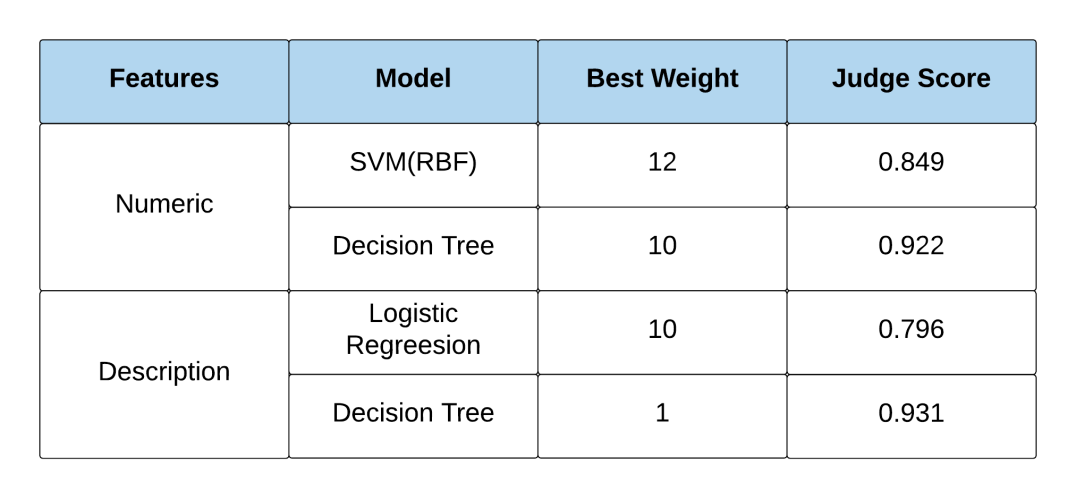
\includegraphics[width=12cm]{figure/classifier_score.png}
    \caption{classifier performance}
    \label{classifier}
\end{figure}


Figure \ref{word_weight} illustrates the words with top weights in SVM-RBF model. Here it only shows stems of words, since we apply Porter Stemming algorithm before load data into database. We can conclude that "Reptile" has the biggest positive score, while "meteor" has the biggest negative score. What surprises us is that "Miami", a state name, is regarded as one of the top positive words. Thus, we are able to make up an UFO event description that is true with high possibility: "a reptile-like alien gets off a cigarette-like spaceship in forest, and all of these are near me." While a fake description probably is: "a meteor-like ship with an alien that is unhuman."
\begin{figure}[H]
    \centering
    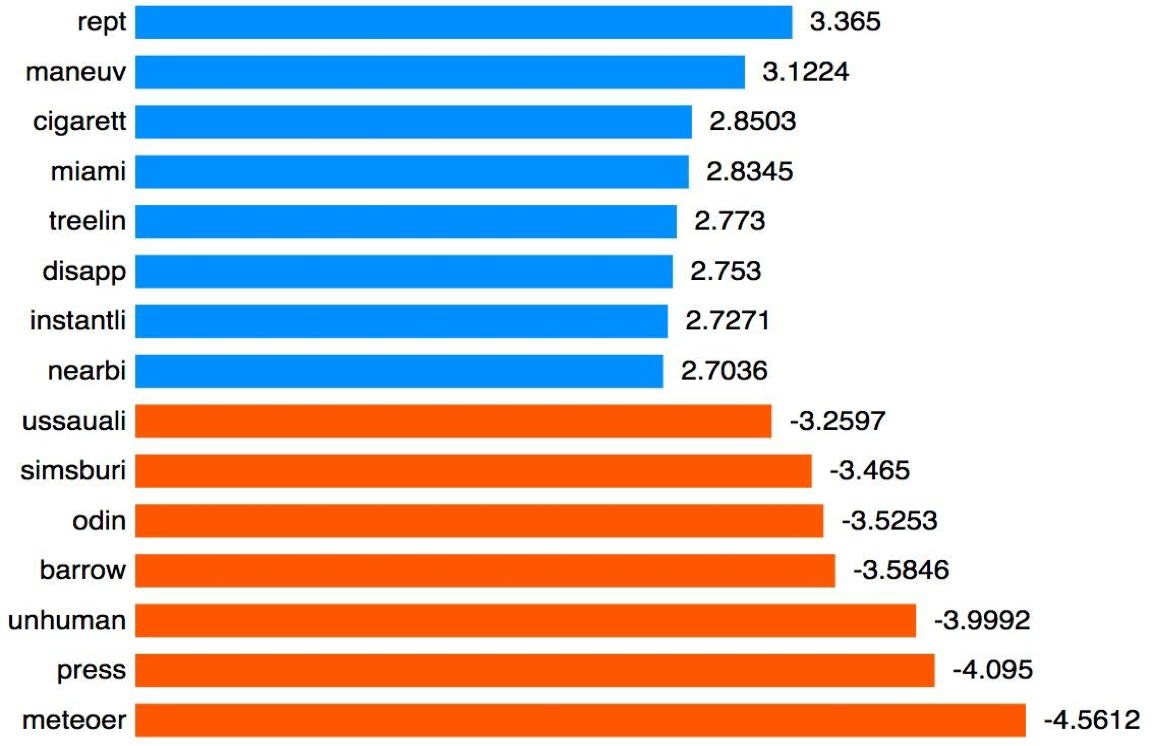
\includegraphics[width=10cm]{figure/word_weight.png}
    \caption{word weight of SVM-RBF}
    \label{word_weight}
\end{figure}

